\documentclass[../../../../main.tex]{subfiles}
\begin{document}

図のように，半径 $a$ の円 $O$ の周を8等分する点を順に $A_1,A_2,\cdots,A_8$ とし，
弦 $A_1A_4$ と弦 $A_2A_7$，$A_3A_6$ との交点をそれぞれ $P$，$Q$ とし，
弦 $A_5A_8$ と弦 $A_3A_6$，$A_2A_7$ との交点をそれぞれ $R$，$S$ とする．

このとき，正方形 $PQRS$ の面積を求めよ．
また，線分 $A_1P$，$A_2P$ と弧 $A_1A_2$ とで囲まれる図形の面積を求めよ．

\begin{figure}[htbp]
  \centering
  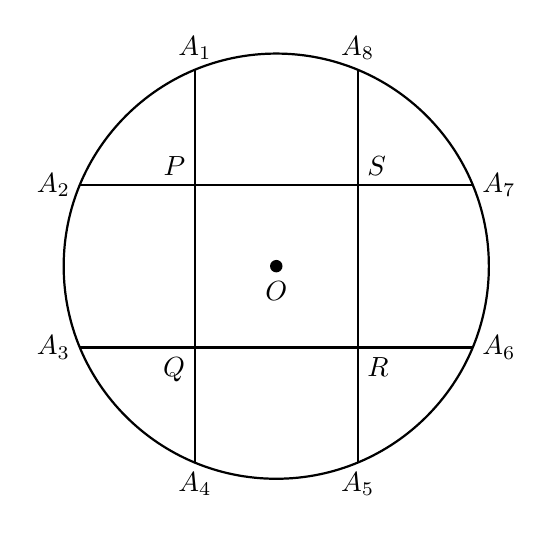
\begin{tikzpicture}[scale=1.5]
    \coordinate (O) at (0,0);
    \draw[thick] (O) circle (1.8);
    \fill (O) circle (1.5pt) node[below=2pt] {$O$};

    \foreach \i/\ang in {1/112.5, 2/157.5, 3/202.5, 4/247.5, 5/292.5, 6/337.5, 7/22.5, 8/67.5} {
      \coordinate (A\i) at (\ang:1.8);
    }

    \draw[thick] (A1) -- (A4);
    \draw[thick] (A8) -- (A5);
    \draw[thick] (A2) -- (A7);
    \draw[thick] (A3) -- (A6);

    \coordinate (P) at (intersection of A1--A4 and A2--A7);
    \coordinate (Q) at (intersection of A1--A4 and A3--A6);
    \coordinate (R) at (intersection of A8--A5 and A3--A6);
    \coordinate (S) at (intersection of A8--A5 and A2--A7);

    \node[above left] at (P) {$P$};
    \node[below left] at (Q) {$Q$};
    \node[below right] at (R) {$R$};
    \node[above right] at (S) {$S$};

    \node[above] at (A1) {$A_1$};
    \node[left] at (A2) {$A_2$};
    \node[left] at (A3) {$A_3$};
    \node[below] at (A4) {$A_4$};
    \node[below] at (A5) {$A_5$};
    \node[right] at (A6) {$A_6$};
    \node[right] at (A7) {$A_7$};
    \node[above] at (A8) {$A_8$};
  \end{tikzpicture}
\end{figure}

\end{document}
